\documentclass[aspectratio=169]{beamer}
\usepackage{pgfpages}
\usepackage{ragged2e}
\usetheme{metropolis}
\setbeameroption{show notes on second screen}

\title{Three Decades of Mustard Watches}
\subtitle{Theory, Practice, and Frontiers}
\date{4 March 2022}
\author{je suis Nezorg}

\begin{document}

\maketitle

\note[itemize]{
\item (introduce myself)
\item will be a short talk, mostly to introduce the topic and invite a discussion on future directions of research in the topic
}

\section{Theory}

\note[itemize]{
\item overview ringard's 1990 paper
\item hope to build intuition through demonstration
}

\begin{frame}{Ringard's Revolution}
    \begin{quote}
    The paper introduces the concept of \textnormal{mustard watch}, a common generalisation of the concepts of watch and of mustard pot. \onslide<2->{The main property of mustard watches is that they can deliver mustard in any desired quantity (theorem 1)} \onslide<3->{and still display time with a precision of 30 seconds (theorem 2).} \onslide<4->{But the real superiority of mustard watches over classical ones is expressed by our theorem 3: a mustard watch with no mustard in it is at least as precise as an ordinary one.}
    \end{quote}

    \note<1>[item]{unfortunately unpublished}
    \note<1>[item]{can badly photocopy my copy if you want} 
    \note<1>[item]{motivations: what is point of time without having mustard?} 
    \note<1>[item]{speculation on how he thought it up: in a bistro, mustard pot was out, difficult to flag down a waiter, so he surveyed what he had on him...} 

    \usebeamercolor[fg]{normal text}
    \begin{flushright}
        ---Yann-Joachim Ringard
    \end{flushright}
\end{frame}

\begin{frame}{Basic Notions}
    \begin{definition}[mustard watch]
        \vspace{1em}
        Let \(W\) be a classical watch; a \emph{mustard watch} derived from \(W\) is any \(W'\) obtained from \(W\) by adding a certain amount of mustard in the mechanism.
    \end{definition}

    \note[item]{watch refers to mechanical wristwatch}
    \note[item]{(now give demonstration)}
    \note[item]{we now have a \emph{proper} mustard watch -- before it was degenerate}
\end{frame}

\begin{frame}{Theorem 1}
    \begin{theorem}[arbitrary mustard]
        \vspace{1em}
        It is possible to get ``as much mustard as wanted'' from a mustard watch. More precisely, given any amount \(m\) of mustard, there is a mustard watch \(W(m)\) containing mustard in quantity \(m\).
    \end{theorem}

    \note[item]{proof: classical watches in any size; take large enough watch for \(m\) consider \emph{completion} of it by adding mustard to it}
    \note[item]{I, among others, are not certain of this proof, considering Ringard's definition of ``watch'' as ``analog pocket watch''; but let us go on}
\end{frame}

\begin{frame}{Theorem 2}
    \begin{theorem}[approximate conservation]
        \vspace{1em}
        A proper mustard watch can display time with a precision of 30 seconds.
    \end{theorem}

    \note[item]{proof: let \(T\) be the current time. reset the watch so that it is within 30 seconds of \(T\). this is possible because the seconds hand of a proper mustard watch is constant, and difference between two seconds values is always less than 30 seconds}
    \note[item]{there are some issues with this proof which ringard himself notes which i will get back to}
\end{frame}

\begin{frame}{Theorem 3}
    \begin{theorem}[superiority]
        \vspace{1em}
        There are mustard watches at least as precise as classical ones.
    \end{theorem}

    \note[item]{Ringard presents a proof using temporal logic \(\Omega 7.2\), which, to be frank, I do not understand the minutae of}
    \note[item]{However, the intuition is roughly that, for any given classical watch \(W\), it is already a degenerate mustard watch; therefore such a mustard watch exists}
\end{frame}

\begin{frame}{Theorem 4}
    \onslide<2->{
    \begin{theorem}[degeneracy of self-metawatches]
        \vspace{1em}
        A mustard watch which is its own metawatch is degenerated.
    \end{theorem}
    }
    \note[item]{foundational issues: theorem 2 proof depends on a metawatch}
    \note[item]{thus would require a predicative hierarchy of metawatches up to \(\omega\)}
    \note<2>[item]{proof intuition: G\"odel's second incompleteness theorem}
    \note<2>[item]{and yet still have decidability of properness! based on the fact that proper mustard watches are silent}
    \note<2>[item]{(hold my mustard watch to my ear)}
\end{frame}

\section{Practice}

\note{very brief, since I know plunch does not care about real-world adoption}

\begin{frame}{Limited Adoption}
    \begin{center}
        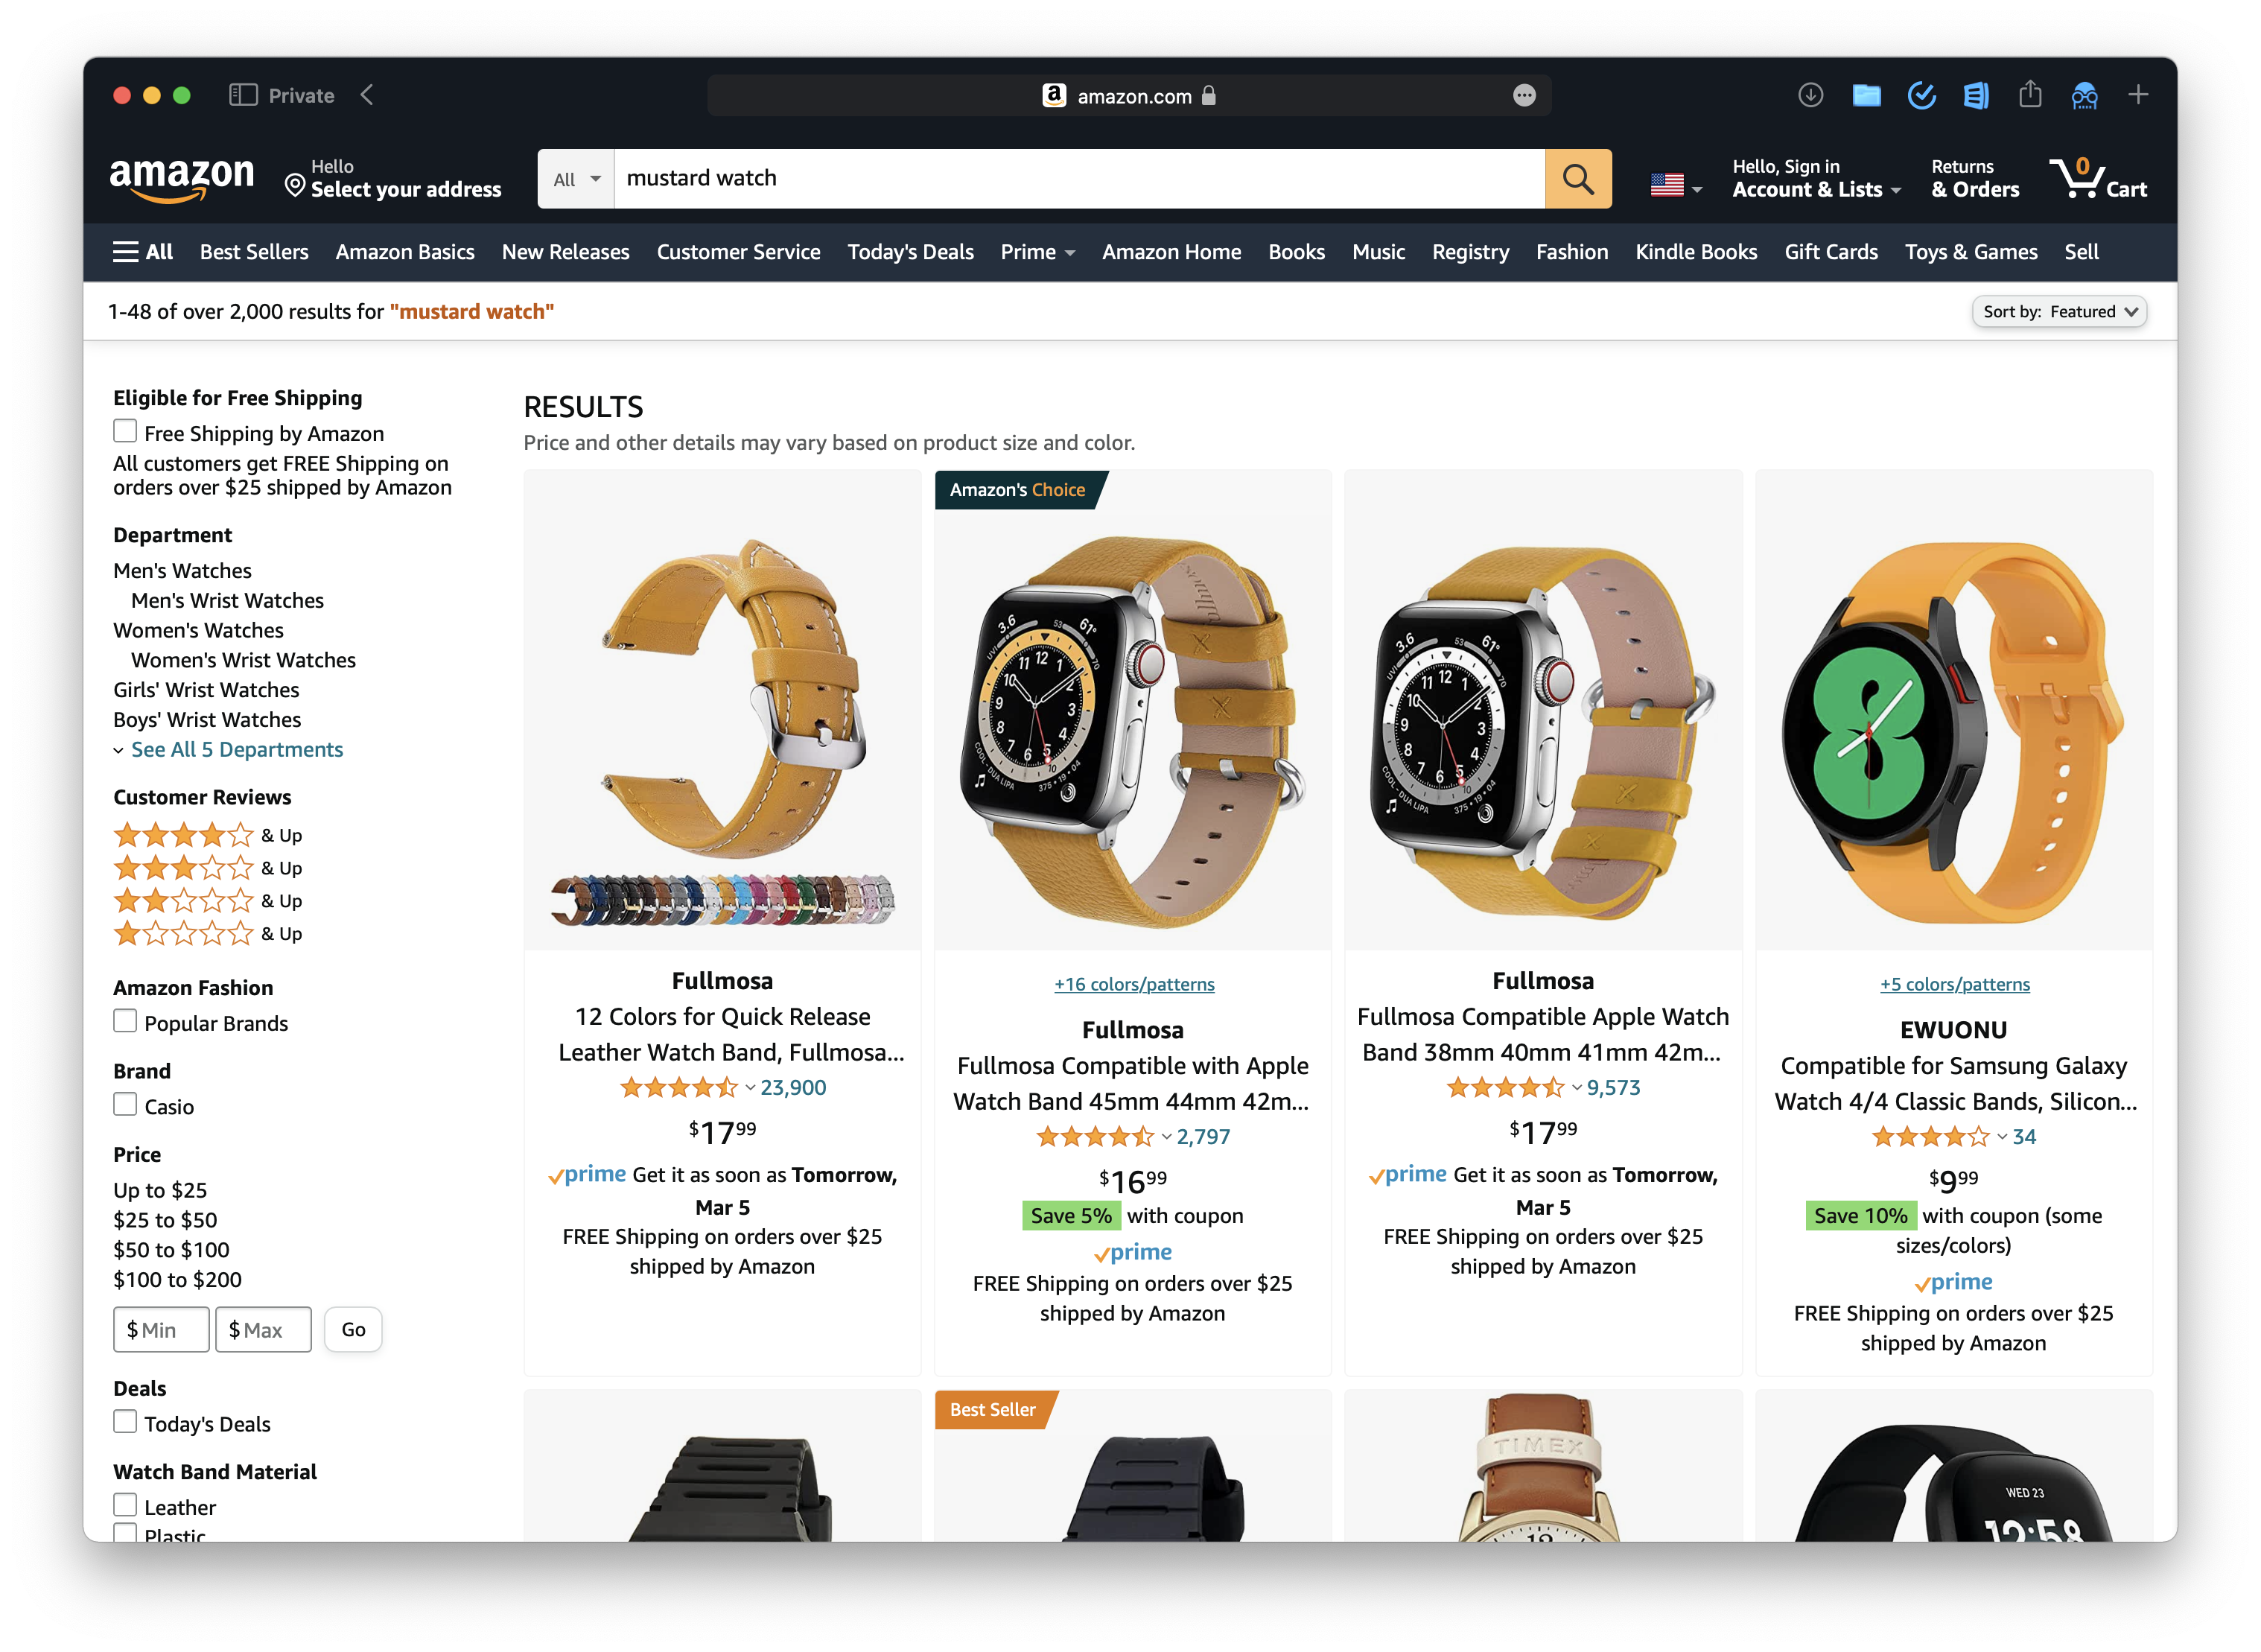
\includegraphics[width=0.7\textwidth]{amazon}
    \end{center}

    \note[item]{unfortuntely limited adoption in industry}
    \note[item]{search in the market turns up only ordinary watches with mustard-colored straps}
\end{frame}

\begin{frame}{Pill ``Watch''}
    \begin{center}
        \includegraphics<1>[width=0.8\textwidth]{pillwatch1}
        \includegraphics<2>[width=0.8\textwidth]{pillwatch2}
    \end{center}

    \note<1>[item]{pill watch, seems inspired by mustard watch}
    \note<1>[item]{initially seems promising}
    \note<2>[item]{...but not actually a watch}
    \note<2>[item]{violates the core principle of mustard watches, that it generalizes both!}
\end{frame}

\section{Frontiers}

\note{overview of some of the current research efforts into mustard watches}

\begin{frame}{Beyond Mustard}
    \begin{columns}
        \begin{column}{0.6\textwidth}
            \centering
            \includegraphics<2->[width=\textwidth]{wholegrain}
        \end{column}
        \hfill
        \begin{column}{0.3\textwidth}
            \centering
            \includegraphics<3>[width=0.3\textwidth]{hotsauce}
        \end{column}
    \end{columns}

    \note<1>[item]{Ringard mentions ketchup watches are clearly ridiculous because you would need too much ketchup, but what about others?}
    \note<2>[item]{Ringard seems to assume a smooth Dijon mustard for some of his constructions -- it is not clear how to fit whole grain mustard into the hole of a mustard watch}
    \note<2>[item]{(demonstrate whole grain mustard)}
    \note<2>[item]{I am currently working on this}
\end{frame}

\begin{frame}{Beyond Watches}
    \begin{columns}
        \begin{column}{0.45\textwidth}
            \centering
            \includegraphics<2->[width=0.3\textwidth]{digital}
        \end{column}
        \hfill
        \begin{column}{0.45\textwidth}
            \centering
            \includegraphics<3>[width=0.8\textwidth]{airpods}
        \end{column}
    \end{columns}
\end{frame}

\begin{frame}[standout]{}
    Beyond mustard watches?
\end{frame}

\note{
    \begin{itemize}
        \item Most in the spirit of Ringard, though, would to be generalize even further, on a third axis!
        \item discussion?
    \end{itemize}
}

\end{document}
